
\chapter{EXPERIMENT 3: AN INVESTIGATION OF RESPONSE BIAS}  \label{ch:exp3}

The previous chapters focused on the role of local ambiguity and response strategies and investigated possible explanations for existing Turkish agreement attraction effects. In those chapters, we have found that the effect of a plural attractor in ungrammatical sentences were not due to a local ambiguity stemming from a case syncretism or a possible form-matching response strategy. Even though both phenomenon have been important aspects of the psycholinguistics literature, it seems that they do not play a role in Turkish agreement attraction given our data and analysis.

Another influential topic in psycholinguistics is the response bias. This chapter aims to investigate the response bias effects in Turkish agreement attraction and try to replicate the results of \citeand{HammerlyEtAl2019}. In addition to our replication, we propose a different calculation of response bias using only fillers, unlike \citeand{HammerlyEtAl2019} who used experimental items. 

\section{Grammaticality asymmetry}
One crucial characteristic of agreement attraction effects that is still under discussion is the grammaticality asymmetry (Acu{\~n}a-Fari{\~n}a, Meseguer, \& Carreiras, 2014; Hammerly et al., 2019; Lago et al., 2021). Consider (\ref{ex:keySgPlSg}) and (\ref{ex:keySgPlPl}), which are minimally different: (\ref{ex:keySgPlSg}) contains a singular verb, thus grammatical, whereas the verb in (\ref{ex:keySgPlPl}) is plural, thus ungrammatical. 

% Maybe include experimental items and shorten them as SgPl etc to use throughout the paper.

\ea
  \ea[]{The {key} to the {cabinets} is rusty. \label{ex:keySgPlSg}}
  \ex[*]{The {key} to the {cabinets} are rusty. \label{ex:keySgPlPl}}
  \z
\z

If agreement attraction were mainly driven by erroneous encoding of the subject, we would expect comparable effects of plural attractor in both grammatical (\ref{ex:keySgPlSg}) and ungrammatical sentences (\ref{ex:keySgPlPl}). However, this is not the case: Studies have found that while there is an effect of plural attractor in ungrammatical sentences, the same effect is not found in grammatical sentences \citep[][among others]{WagersEtAl:2009,LagoEtAl2015,LagoEtAl2019,JagerEtAl2020}. That is, we do not see an ungrammaticality illusion in grammatical sentences that contain a plural attractor. Participants do not accept grammatical sentences with plural attractor less often compared to their singular attractor counterpart. Moreover, there seems to be no substantial RT difference between singular and plural attractor conditions in grammatical sentences.

These findings pointed towards an understanding of agreement attraction in which the attraction is a result of a retrieval process triggered by the verb and is not due to the erroneous representation of the subject head. Because of this, these accounts assume that dependencies are satisfied via matching cues ({Case} and {Number}) of the verb with features of the DP. Thus, they predict that participants successfully retrieve the subject in grammatical sentences since the retrieval process is not hindered due to any mismatching cue-feature pair. 

However, when the verb and the subject head have different number marking, meaning that the sentence is ungrammatical, all cues provided by the verb ({Case} and {Number}) cannot fully match the features of the subject DP, only the case feature is satisfied. However, participants may entertain other DPs that partially match the provided cues ({Number} but not {Case}). In these cases, these DPs may interfere with the subject-verb dependency and be erroneously retrieved by the verb as an agreement controller. These erroneous retrievals, often referred as attraction effects, only occurs in ungramatical sentences. 

Recently, a study by \citeand{HammerlyEtAl2019} has shown that the grammaticality asymmetry may not be due to the intricacies of memory retrieval and the processing of the agreement attraction. Instead, they argue that it is a result of participants' inclination to give yes responses more often. 

Following the Drift-Diffusion Model introduced by \citeand{Ratcliff1978}, they argued that participants' default state is biased towards deciding that sentence is grammatical, rather than a neutral state in which participants judge every sentence without any prior expectation. According to their analysis, this bias towards grammaticality is the driving force behind the lack of attraction effects in grammatical sentences. Through instructions and the proportion of ungrammatical sentences, they manipulated the overall response bias of the participants. They found that participants made substantially more errors in grammatical sentences with plural attractor when their response bias towards grammatical responses was reduced. Their findings challenged the notion of grammaticality asymmetry and provided evidence for theories that do not explain agreement attraction effects through retrieval mechanisms.



\section{Response bias and agreement attraction} \label{sec:ddm}

Imagine a selection committee that needs to decide whether or not to recruit people based on prospective employees' backgrounds. Even though all information provided is the same, committee members' decisions are different. Certain members decide on recruiting people most of the time. The reason why they mostly choose to recruit people may be due to several reasons. One possibility may be the fact that those members have an overall tendency to accept people rather than reject when there is no clear answer to give or in situations where they are uncertain. This phenomenon, known as response bias, is the tendency to choose one alternative over another possible candidate given a certain amount of time \citep{GreenSwets1966, MacmillanCreelman2005}. 

One cognitive model that accounts for people's bias is \cites{Ratcliff1978} drift-diffusion model, shown in a simplified manner in Figure \ref{fig:diffusionmodel}. \citeauthor{Ratcliff1978} develops a cognitive model which assumes that noisy information is accumulated over time following a Gaussian distribution whose mean is linearly correlated with the stimulus strength. The information accumulation is terminated, and a decision is made when either of the thresholds is reached, representing two choices.

\begin{figure}[hbt!]
  \centering
  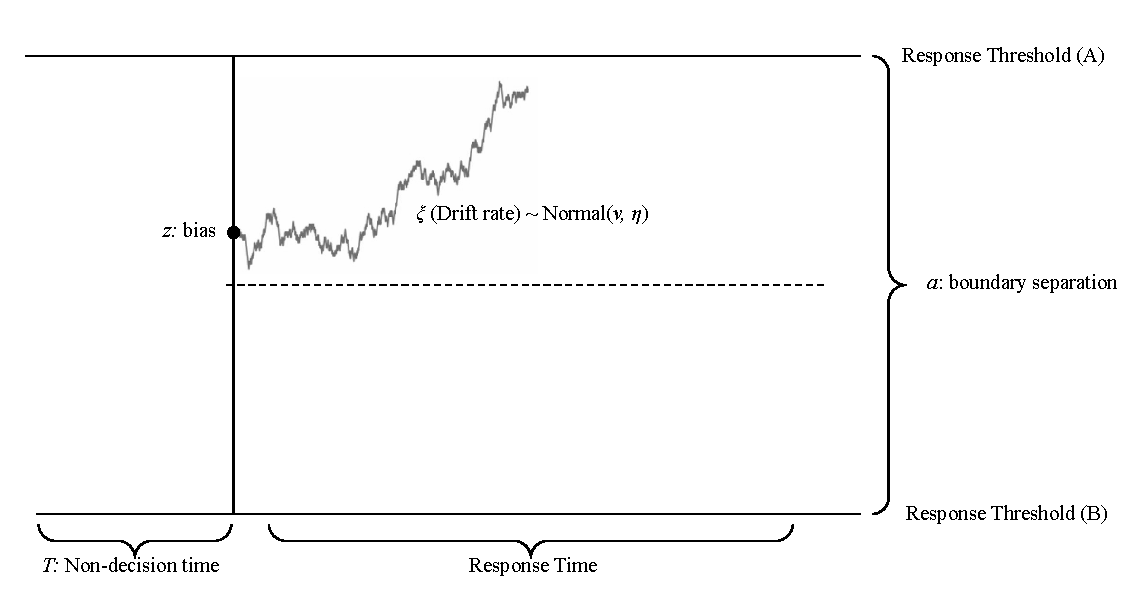
\includegraphics[width=\textwidth]{figure/ddm_model_grey.pdf}
  \caption{Simplified illustration of the drift-diffusion model. On every trial, after a period of time (T), an evidence accumulation process is initiated from the specified position (z) relative to the whole boundary separation (a). Evidence is gathered stochastically according to the drift rate ($\xi$) that follows a normal distribution with the mean v and the standard deviation $\eta$. When enough information is accumulated to cross one of the thresholds, a decision is made}
  \label{fig:diffusionmodel}
\end{figure}

Among five parameters shown in Figure \ref{fig:diffusionmodel} that govern the model's predictions, the starting point of information accumulation is the interest of this paper. The a priori bias of the participants can be defined as this starting position relative to decision thresholds, represented with \emph{z}, \emph{A}, and \emph{B} in Figure \ref{fig:diffusionmodel}. For example, suppose that the response bias (\emph{z}) is equal to half the distance between response thresholds (\emph{a/2}). In that case, we assume that participants do not have a bias towards either of the thresholds, and the decision to be made will be mainly determined by the drift rate \emph{$\xi$} --- the quality of stimuli's information. According to the model, as we increase the \emph{z} and hold the other parameters constant, we should see an overall increase in the number of A answers and a decrease in response times of A answers. On the other hand, if we decrease the \emph{z} with other parameters being constant, we expect an overall decrease in A answers and an increase in their response times.

An acceptability judgment task, a forced two-choice experiment, can also be conceptualized as a diffusion process. Possible answers, `acceptable' and unacceptable, can be represented as the upper and lower thresholds, respectively. \citeand{HammerlyEtAl2019}, building on \cites{Staub2009} work, proposed an implementation of the drift-diffusion model to the agreement attraction phenomenon and Marking and Morphing account. They hypothesized that as the response bias, starting position of the evidence accumulation, decreases, the acceptable responses to grammatical sentences should also decrease. Furthermore, this decrease should be sharper when there is a plural attractor due to its influence on the drift rate. Their argumentation follows from the Marking and Morphing account, where the agreement attraction effects surface due to the erroneous representation of the subject, and this representation is formed before the processing of the verb. Thus, the presence of a plural attractor should have the same effect in both grammatical and ungrammatical sentences.

On the other hand, in the cue-based retrieval model, the agreement attraction results from erroneous retrieval of the agreement controller when there is no single match to the cues provided by the verb. Thus, it should surface only in ungrammatical sentences, and the presence of the plural attractor should not influence the drift rates. When a participant's response bias changes, there should not be any effect of the plural attractor in grammatical sentences under the cue-based retrieval account of agreement attraction. These details are visualized in Figure \ref{fig:ddmSimulation}. 


\begin{knitrout}
\definecolor{shadecolor}{rgb}{0.969, 0.969, 0.969}\color{fgcolor}\begin{figure}[hbt!]

{\centering 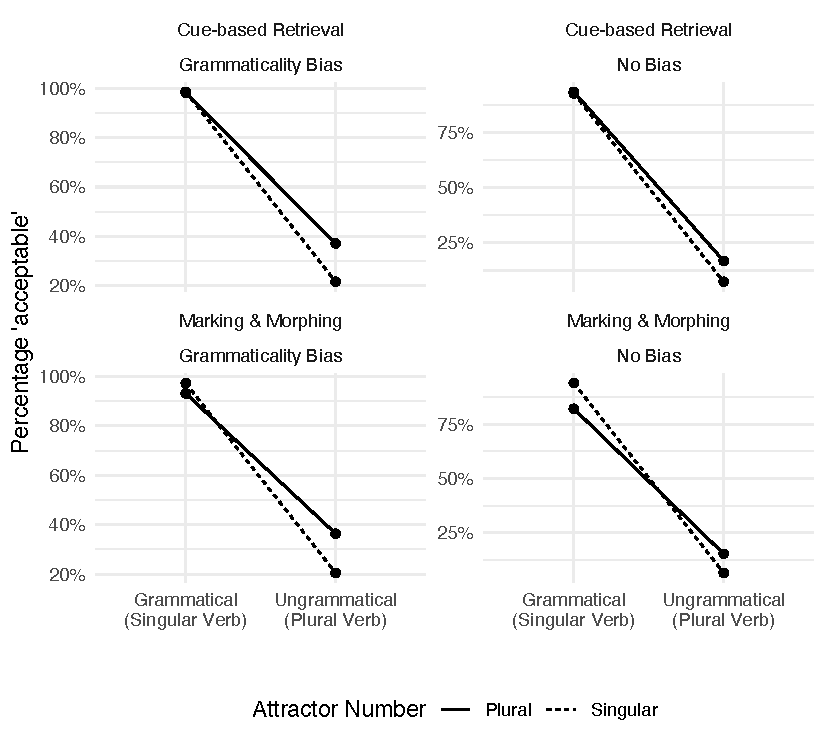
\includegraphics[width=\linewidth]{figure/ddmSimulation-1} 

}

\caption{Drift Diffusion Model predictions in which the drift rate is manipulated according to the assumptions of agreement attraction accounts along with a bias manipulation}\label{fig:ddmSimulation}
\end{figure}

\end{knitrout}


As it can be seen from Figure \ref{fig:ddmSimulation}, there is no effect of the plural attractor in grammatical sentences under the cue-based retrieval account in either bias condition. On the other hand, we see a clear difference in the influence of plural attractor depending on the bias manipulation under Marking and Morphing account. This difference follows from the fact that readers should first detect the ungrammaticality and only then consider the attractor as a candidate for the agreement under the cue-based retrieval account. In contrast, readers may be influenced by the plural attractor regardless of grammaticality under Marking and Morphing account.

When \cites{HammerlyEtAl2019} findings are compared to the visualization in Figure \ref{fig:ddmSimulation}, we see that their data is more compatible with Marking \& Morphing theories where the effect of sentence grammaticality is substantially reduced. Furthermore, the effect of the attractor number is roughly the same across the board. However, their manipulation of bias and results were only in English in a single experiment, which calls for a replication study in another language.

\section{Experiment 3}

In this chapter, we seek to clarify the status of the response bias in agreement attraction. We aim to replicate \cites{HammerlyEtAl2019} findings in another language, Turkish, with a different syntactic construction. To this end, we conducted a speeded acceptability judgment task with two within-subject manipulations (attractor number x verb number) and a between-subject manipulation (bias) which we introduced through instructions and the ratio of ungrammatical sentences as \citeand{HammerlyEtAl2019} did. We focus on number agreement attraction using an atypical structure, complex NP with a non-intervening genitive modifier. Both \citeand{LagoEtAl2019} and our Experiment 1 have established that these structures as in (\ref{ex:lago}) are prone to attraction effects.

\ea \label{ex:lago} 
  \gll {Milyoner-\{\O/ler\}-in} {terzi-si} tamamen gereksizce kov-ul-du-\{\O/lar\}.\\
  millionaire-\{\Sg/\Pl\}-\Gen{} tailor-\Poss{} completely without\_reason fire-\Pass-\Pst\{.\Tsg/-\Tpl\}\\
  \glt `The millionaire's/millionaires' tailor were fired\{\Sg/\Pl\} for no reason at all.'
\z

Considering our results in Experiments 1, 2A, and 2B, we conclude that agreement attraction effects in Turkish with an atypical syntactic structure are replicable. Building on this work, we sought to test the predictions of a drift-diffusion model and how the bias manipulation proposed by \citeand{HammerlyEtAl2019} would affect agreement attraction effects in grammatical sentences in Turkish. We reasoned that \cites{HammerlyEtAl2019} data, manipulation, and findings should be replicated, given that the Drift Diffusion model account of decision making is not limited to a particular language, a particular structure, or a particular demographic.



\subsection{Participants}

114 Turkish speakers participated in the experiment. All participants were recruited through Bo\u{g}azi\c{c}i University in exchange for course credit. Because 3 participants indicated that Turkish is not their first language, we excluded their data from the analysis. Participants had an average age of 20 (range: 29 - 18). The experiment was carried out following the principles of the Declaration of Helsinki and the regulations concerning research ethics at Bo\u{g}azi\c{c}i University. Before the experiment, all participants were explicitly asked for their consent and informed with respect to their rights. All sensitive information about the participants is anonymized.


\subsection{Materials}

In our study, we used the same experimental items that we used in our Experiment 1. 


In our experiment, all experimental sentences with a singular verb are grammatical, and all sentences with a plural verb are ungrammatical. Due to this distribution, we speculated that participants might form a strategy in which they automatically judge sentences ungrammatical when they see a plural ending. To this end, we created 60 filler items, half of which consist of ungrammatical sentences with singular marked verbs (\ref{ex:ungFiller}). In contrast, the other half is grammatical sentences with plural verbs (\ref{ex:grFiller}). 

Another purpose of the fillers was to manipulate participants' response bias. Along with the instructions, we have manipulated the number of grammatical and ungrammatical fillers in the experiments following \citeand{HammerlyEtAl2019}. We created two sub-experiments with two different ratio of ungrammatical stimulus. In the first sub-experiment, we intended to shift participants' bias towards ungrammatical responses by using only 10 grammatical fillers and 20 ungrammatical fillers. In the second sub-experiment, we wanted participants to have a bias towards grammatical responses. To ensure this, we used only 10 ungrammatical fillers and 20 grammatical fillers.

Most filler items started with a genitive-possessive NP similar to experimental items. However, this initial NP was not the subject of the main sentence but the subject of an embedded adverbial clause. In grammatical fillers (\ref{ex:grFiller}), we used a plural-marked verb whose subject is pro-dropped following the verb of the embedded adverbial clause. In ungrammatical fillers (\ref{ex:ungFiller}), we used a transitive verb whose non-local object lacked the case marking, making the sentence ungrammatical. While most of the fillers followed a strict template, 20 of the 60 were with no particular order, and half of them were grammatical sentences  with plural verbs (N=10) and the other half were ungrammatical sentences (N=10) with singular verbs. All of our experimental and filler items can be found in Appendix \ref{ap:exp3items}.


\ea \label{ex:fillers}
  \ea {Ungrammatical Filler} \label{ex:ungFiller}\\*
  \gll \"O\u{g}renci-nin hoca-s{\i} ayr{\i}l-{\i}nca proje birden unut-tu.\\
  student-\textsc{gen} teacher-\textsc{poss} leave-\textsc{when} project suddenly forget-\textsc{pst}\\
  \glt Intended: `Suddenly, he forgot the project when the student's professor left.'
  \ex {Grammatical Filler} \label{ex:grFiller}\\*
  \gll Patron-un yeme\u{g}-i yer-e d\"ok-\"ul-\"unce yeni-sin-i yap-t{\i}-lar.\\
  boss-\textsc{gen} meal-\textsc{poss} floor-\textsc{dat} spill-\textsc{pass}-\textsc{when} new-\textsc{poss}-\textsc{acc} do-\textsc{pst}-\textsc{pl}\\
  \glt `They prepared a new one when boss' meal spilled on the floor.'
  \z
\z





Before our experimental study, we ran a speeded acceptability judgment study where participants (N = 8) saw all experimental and filler items. Experimental items were distributed among four different lists according to a Latin Square design. One of the main reasons for conducting the norming study was to find the most acceptable grammatical and the least acceptable ungrammatical fillers for the Bias manipulation. We only used the ten least acceptable ungrammatical fillers to shift the response bias towards grammatical responses. Similarly, we only used the ten most acceptable grammatical fillers to shift the bias towards ungrammatical responses. We also wanted to check the overall acceptability of our grammatical items with singular attractor and confirm that there was no problem with the baseline sentences. We confirmed that our grammatical experimental items with singular attractor were found grammatical with no problem (M = 0.99, SE = 0.01). 

\subsection{Procedure}

The experiment was run online, using the web-based platform Ibex Farm \citep{Drummond2013}. Each experimental session took approximately 30 minutes to complete. After the first page participants landed, they were randomly assigned to one sub-experiment that incorporated the between-subject bias factor. Prior to the experiments, participants were asked to give informed consent to participate in the experiment. They then read the instructions, which included four already answered example sentences. After the instructions, they were given nine practice trials before the experiment began. After they finished practice trials, participants were prompted with a message stating the distribution of the sentences and asked to confirm that they understood the statement. The instructions are as follow:


\ea \label{ex:biasManip}
  \ea \label{ex:biasUngManip} {Ungrammaticality Bias Condition}\\*
  Bu deneydeki c\"umlelerin \c{C}O\u{G}U T\"urk\c{c}e kurallar{\i}na UYMAMAKTADIR!\\*
  `MAJORITY of sentences in this experiment DO NOT FOLLOW the rules of Turkish.'
  \ex \label{ex:biasGrManip} {Grammaticality Bias Condition}\\*
  Bu deneydeki c\"umlelerin \c{C}O\u{G}U T\"urk\c{c}e kurallar{\i}na UYMAKTADIR!\\*
  `MAJORITY of sentences in this experiment DO FOLLOW the rules of Turkish.'
  \z
\z

After participants were informed concerning the distribution of sentences' grammaticality, experiment was initiated in the IbexFarm. Each trial began with a blank screen for 600 ms, followed by a word-by-word RSVP presentation of the sentence in the center of the screen. Sentences were presented word-by-word in the center for the screen in 30 pt font size, at a rate of 400 ms per word. Participants saw a blank screen for 100 ms between each word, and to see the next item, they needed to press the space key. After every trial, participants are asked to indicate their acceptability judgment. The wording of the question is given in (\ref{ex:question}). 

\ea \label{ex:question}
Bu c\"umle kula\u{g}{\i}n{\i}za nas{\i}l geliyor? \\*
`How does this sentence sound to you?'
\z

The possible answers that participants could provide were either good or bad. Participants were asked to press the key P to indicate that a sentence is acceptable/good and Q to indicate that the sentence is unacceptable/bad. Within instructions before the experiments, they were told to provide judgments as soon as possible. If they did not respond within 5,000 ms during the experiment, the trial timed out, and participants were shown message `\emph{Please respond faster,}' in a red font.

Participants saw 40 experimental and 40 filler sentences. Experimental sentences were distributed among four different lists according to a Latin-square design. Every participant saw one version of the experiment with a specific list and one item per condition while seeing all filler items in that specific between-subject condition.


\subsection{Analysis}


The experimental data were collected from the IbexFarm website in a csv file format and imported to R for data cleaning, visualization, aggregation, and analysis. 

We excluded all 3 participants whose native language was not Turkish in the data cleaning process. Moreover, we removed the data for all participants who did not show sufficient sensitivity to the grammaticality in singular attractor conditions. Specifically, we excluded all participants whose difference in percentages of acceptable responses in grammatical sentences with singular attractors and ungrammatical sentences with singular attractors fell below 0.25 percentage points. Finally, we also excluded trials in which the participants missed the response deadline or gave too fast responses (below 200 ms). As a result, 9.05\% of trials were excluded from our experiment. 

% In Figure \ref{fig:MissingDataPlot}, you can see that the percentage of missing data or exclusion due to given RT and accuracy criteria compared to the total amount of data. Since the number of missing values and exclusions is quite small, we decided to ignore them and treat the data as missing completely at random. Due to this outcome, we treat them as they are irrelevant to the rest of the data.

% \begin{figure}[hbt!]
%   \centering
  
% <<MissingDataPlot,  echo=FALSE, fig.align='center', height=3, warning=FALSE,  dpi = 600, message=FALSE>>=

% missingdata_plot

% @
%   \caption{}
%   \label{fig:MissingDataPlot}
% \end{figure}




While reporting the aggregated details of the experimental data, we have used the categorical bias grouping we introduced following calculated bias values instead of our experimental manipulation. We calculated means and standard errors using tidyverse packages. In calculating the standard errors, we followed \citeand{Morey2008} and \citeand{Cousineau2005}. 


Since our research question is whether the change in bias affects acceptability in ungrammatical sentences and grammatical sentences, we grouped our responses according to the grammaticality of the sentences. We only use the ungrammatical sentences to see the already acknowledged agreement attraction effects. We then fitted another model, where we used only grammatical sentences to see the possible interaction between the plural attractor and the bias shift. We used the R packages brms \citep{R-brms_a,R-brms_b} and rstan \citep{R-rstan} to fit Bayesian hierarchical models \citep[e.g.,][]{GelmanHill:2007,NicenboimVasishth:2016}.

We fitted two Bayesian GLMs to yes responses as a function of the following predictors: (i) logarithm of the trial number (\emph{log}(trial)), (ii) sum-coded (0.5 vs. -0.5) attractor number (Pl.Attr.), (iii) continuous response bias value \emph{c} (Bias), along with two-way interaction of Pl.Attr. and Bias. We assumed that acceptable responses are distributed following a Bernoulli distribution with a probit-link function. We included only the experimental sentences in our analysis. Our models included maximal random-effect structures to the extent that our design justified. It allowed predictors in interest to vary by-participant (Pl.Attr., Bias) and by-item (Pl.Attr., Trial). The same priors from Experiment 1 is also used in these models. Our first model included only ungramatical sentences, while the second one included only grammatical sentences. Apart from this difference, all model specifications were the same.

\subsection{Bias Calculation} \label{sec:bias}

Before further statistical analysis, we wanted to test whether or not our bias manipulation was successful. Therefore, we calculated response bias value \emph{c} by participant, using equation (\ref{eq:bias}) \citep{MacmillanCreelman2005}. 

\begin{equation} \label{eq:bias}
c = -\frac{Z(Hit{\ }Rate)+Z(False{\ }Alarm{\ }Rate)}{2}
\end{equation}

Unlike \citeand{HammerlyEtAl2019}, we used only filler sentences in our response bias calculation. The reason for using only fillers is that we wanted to calculate response bias independently of the agreement attraction patterns. Since experimental items may be affected by either a grammaticality illusion or an ungrammaticality illusion, we believe using experimental items would create confounded results.

Figure \ref{fig:OurBiasBFPlot} shows the average bias value of participants in our experiment. We calculated the response bias using both only experimental items (\cites{HammerlyEtAl2019} way) and only filler items. On the x-axis, we indicate our manual bias manipulation, which also shown with different line types. As shown in Figure \ref{fig:OurBiasBFPlot}, our bias manipulation was not successful. The calculation using experimental items shows that there is a bias difference however it is reverse of what we originally intended. The calculation using filler items shows that both distributions heavily overlap and there is no difference in terms of participants' bias. We expected a significant bias towards grammatical responses (negative \emph{c}) in the grammaticality bias condition (Towards Yes). We also expected substantially more positive response bias values in the ungrammaticality bias condition. 


\begin{knitrout}
\definecolor{shadecolor}{rgb}{0.969, 0.969, 0.969}\color{fgcolor}\begin{figure}[hbt!]

{\centering 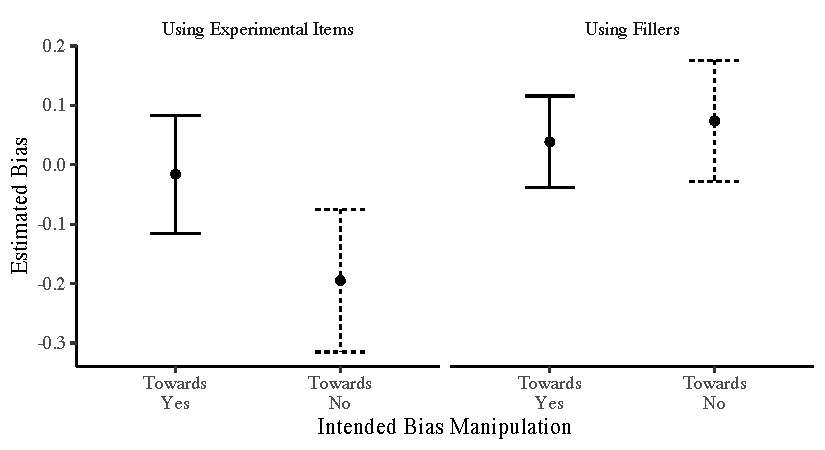
\includegraphics[width=\linewidth]{figure/OurBiasBFPlot-1} 

}

\caption{The average bias value in our Experiment 3 as a function of our intended bias manipulation and different calculation methods. The error bars indicate 95\% credible intervals. The negative \emph{c} values indicates a bias towards yes responses. The estimates in the left sub-figure are calculated with the experimental items only, while the estimates in the right sub-figure with filler items}\label{fig:OurBiasBFPlot}
\end{figure}

\end{knitrout}

We also calculated the Bayes Factor in favor of the hypothesis of no difference between grammaticality and ungrammaticality bias conditions using the statsExpressions package \citep{statsExpressions}. We deployed a one-sided Bayesian hypothesis test with an uninformative JZS Cauchy prior with the scale parameter $1.41$, which is specified by the statsExpressions package. It revealed that given the data, the null hypothesis (no difference) is eight times more likely (moderate evidence) than the alternative hypothesis of a significant difference between grammaticality and ungrammaticality response bias manipulation (BF$_{01}$ = 8, $\delta_{difference}^{posterior}$ = 0.03, CI$_{95\%}^{HDI}$ = [-0.09, 0.16], $r_{cauchy}^{JZS}$ = 1.41).

Given the distribution of our participants and the BF score, it is clear that participants did not respond to our bias manipulation.
We would expect to find at least moderate evidence towards the alternative model if our manipulation were successful. Graphically speaking, we would expect most of the subject points in the grammaticality bias condition to reside in the negative values, which was not the case.

In addition to our own results, we also computed the bias value of \cites{HammerlyEtAl2019} experiments using only the fillers for better comparison. In Figure \ref{fig:HammerlyBias}, we present the participants' estimated response bias following their method of calculating bias (through experimental items alone) as well as ours (through filler items alone). 


\begin{knitrout}
\definecolor{shadecolor}{rgb}{0.969, 0.969, 0.969}\color{fgcolor}\begin{figure}[hbt!]

{\centering 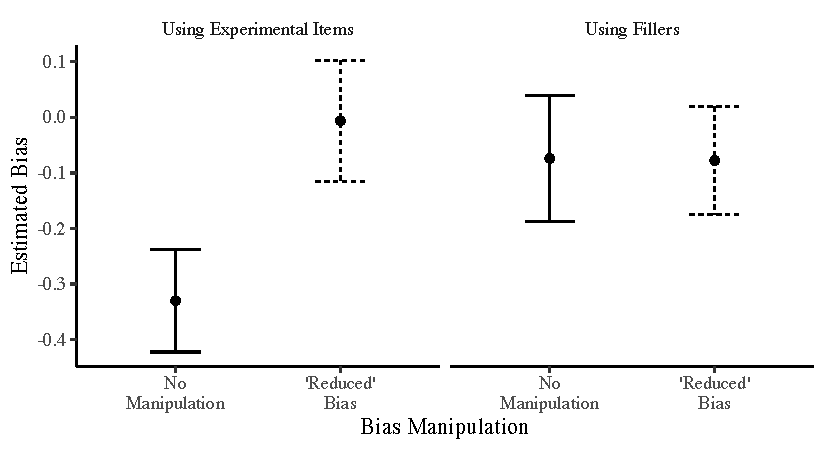
\includegraphics[width=\linewidth]{figure/HammerlyBias-1} 

}

\caption{The average bias value in \cites{HammerlyEtAl2019} study as a function of our intended bias manipulation and different calculation methods. The error bars indicate 95\% credible intervals. The negative \emph{c} values indicates a bias towards yes responses. The estimates in the left sub-figure are calculated with the experimental items only, while the estimates in the right sub-figure with filler items}\label{fig:HammerlyBias}
\end{figure}

\end{knitrout}
%Box plot of by-experiment response bias estimates with individual subject points from \cites{HammerlyEtAl2019} study. Box plots show the median value and first and third quartiles. Negative response bias signals a bias towards grammatical responses, while positive values mean a bias towards ungrammatical responses. The estimates in the sub-figure A are calculated with the experimental items only, while the estimates in the sub-figure B with filler items.

In their work, \citeand{HammerlyEtAl2019} state that they were able to manipulate the response bias between their experiments. 
We replicated their calculation and summary of response bias in the left-side of Figure \ref{fig:HammerlyBias} using experimental items. 
Our Bayesian hypothesis test suggests that given the data, the alternative hypothesis of a significant difference between grammaticality and ungrammaticality response bias manipulation is 1053 times more likely (extreme evidence) than the null hypothesis of no difference (BF$_{01}$ = 1/1053, $\delta_{difference}^{posterior}$ = 0.31, CI$_{95\%}^{HDI}$ = [0.18, 0.46], $r_{cauchy}^{JZS}$ = 1.41).

However, we argued that experimental items should not be included in the calculation of the response bias.
When only experimental items are used, the hit rate corresponds to the mean accuracy of grammatical conditions, including grammatical sentences with plural attractors. 
This means if there is an effect of a plural attractor in the grammatical conditions due to possible agreement attraction effects, let us say decreased accuracy, the response bias value will also be affected.
Similarly, the false alarm rate calculation will also be affected by the agreement attraction effect assuming that participants exhibit classic agreement attraction effects in ungrammatical sentences.
%Moreover, regardless of the item type, be it experimental or filler, participants' response bias should be reflected in their proportion of correct answers. 
For these reasons, we believe that their reported response bias summary using experimental items does not reflect the response bias truthfully and is affected by the agreement attraction effects present in their results.

When we use a calculation method that is not confounded with the agreement attraction effects, as in the right-side of Figure \ref{fig:HammerlyBias}, we see that the bias distribution among participants changes substantially, and there is no longer a significant difference between groups. 
Given the data, the null hypothesis of no difference between grammaticality and ungrammaticality response bias manipulation is eight times more likely (moderate evidence) than the alternative hypothesis of significant difference (BF$_{01}$ = 8, $\delta_{difference}^{posterior}$ = -0.00378, CI$_{95\%}^{HDI}$ = [-0.14, 0.14], $r_{cauchy}^{JZS}$ = 1.41).

Focusing only on the bias distribution based on the filler items, 
we see that participants were not responsive to the bias manipulation implemented by the researchers 
both in \cites{HammerlyEtAl2019} study and our study. 
Since \cites{HammerlyEtAl2019} findings were reliant on the fact that they manipulated the response bias, and participants' exhibited ungrammaticality illusions only with the change of the response bias, 
our re-evaluation of the response bias calculation cast a shadow on their findings and claims on the processing of agreement attraction. 
However, we were still able to test the theoretical claims of \citeand{HammerlyEtAl2019}: participants are biased towards grammatical responses, and as participants' response bias is shifted towards ungrammatical responses, they exhibit ungrammaticality illusions, i.e. an affect of plural attractor in grammatical sentences. 
To test this claim, we divided participants into two groups according to their calculated bias value \emph{c}. 
If the \emph{c} value is negative, we classified those participants as biased towards grammatical answers. 
If it was positive, they were treated as biased towards ungrammatical answers. 
We also included the continuous bias value for each participant to our Bayesian GLMs in all subsequent analyses.


%But we have very limited number of ungrammatical fillers. what if we also include singular attractor items in bias manipulatio as well?




\subsection{Results}

In this section, we provide summaries of the coefficient posterior distributions. We ran 4 chains with 1000 warm-up iterations and 4000 sampling iterations for our models. Our results report the posterior probability of the effect of coefficient $\beta$ being outside of the ROPE region, either smaller than $-0.1$ (\emph{P}($\beta < -0.1$)) or bigger than $0.1$ (\emph{P}($\beta > 0.1$)). If a distribution is completely outside of this area, we can say that we have definitive evidence for an effect. If it covers the practical equivalence area, we can say that according to our data, there seems to be no evidence for an effect. On occasions in which only a part of the distribution resides in the area, we explicitly quantify our degree of belief towards an effect. 



Accuracy in our fillers was relatively high with an average of 0.81 and standard error of 0.02 in participants with grammaticality bias and 0.81 and a standard error of 0.01 in participants with ungrammaticality bias. In Figure \ref{fig:FillerAverage}, we can see the individual means and standard errors according to the experimental conditions {bias} (on the x-axis) and {Grammaticality} (as a line type).


\begin{knitrout}
\definecolor{shadecolor}{rgb}{0.969, 0.969, 0.969}\color{fgcolor}\begin{figure}[hbt!]

{\centering 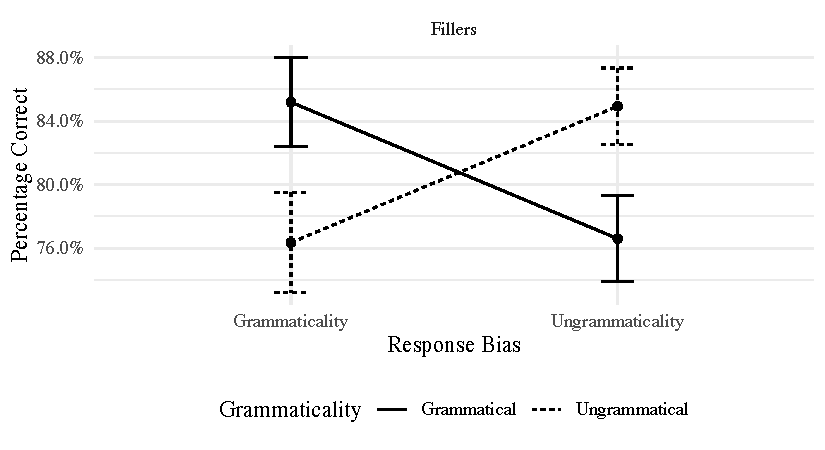
\includegraphics[width=\linewidth]{figure/FillerAverage-1} 

}

\caption{The average accuracy of fillers in Experiment 3}\label{fig:FillerAverage}
\end{figure}

\end{knitrout}
%The average accuracy of fillers in our study. Error bars signal standard errors calculated following \citet{Morey2008} and \citet{Cousineau2005}.


Figure \ref{fig:AvgResponse} shows the average proportions of acceptable responses in each of the eight conditions. Since we are interested in how bias affects the difference in acceptability between grammatical and ungrammatical sentences and the plural attractor interacts with this difference, we grouped the averages into facets according to the grammaticality of the sentences. While the x-axis shows the categorical bias grouping, which we introduced following calculated bias values, the line type shows the attractor number. We see that, on average, participants gave more acceptable responses in ungrammatical sentences with ungrammaticality bias (M = 0.08, SE = 0.01) rather than grammaticality bias (M = 0.2, SE = 0.02). More importantly for us, participants with ungrammaticality bias make more errors in grammatical sentences with plural attractors (M = 0.88, SE = 0.02) compared to the ones with singular attractors (M = 0.93, SE = 0.01). This effect of attractor number is not present in grammatical sentences when the participants have a grammaticality bias.


\begin{knitrout}
\definecolor{shadecolor}{rgb}{0.969, 0.969, 0.969}\color{fgcolor}\begin{figure}[hbt!]

{\centering 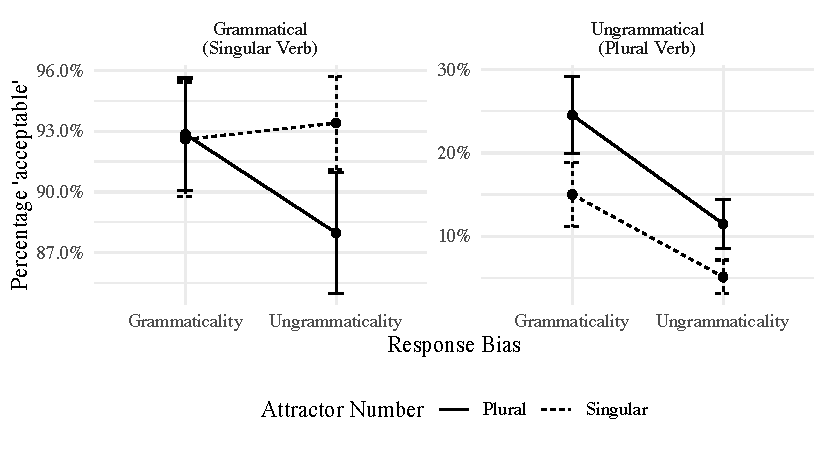
\includegraphics[width=\linewidth]{figure/AvgResponse-1} 

}

\caption{The average percentage of acceptable responses according to the experimental conditions in Experiment 3}\label{fig:AvgResponse}
\end{figure}

\end{knitrout}
%The average percentage of acceptable responses according to the experimental conditions in our study. Error bars signal standard errors calculated following \citet{Morey2008} and \citet{Cousineau2005}.

In Figure \ref{fig:UngramaticalBayesianGLM}, we see the posterior probabilities for our Bayesian GLM model with a probit link, in which we only use ungrammatical sentences. The negative main effect of ungrammaticality bias ($\hat{\beta}=-1.14;$ $CI=[-1.67; -0.61];$ $P(\beta>0.1)< .001$) indicates that, on average, participants gave less acceptable responses as their bias (calculated through fillers) shifted towards ungrammaticality. This verified that our bias calculation using fillers was effecting given that the effect is also present in experimental items. Additionally, the positive main effect of the plural attractor ($\hat{\beta}=0.47;$ $CI=[0.26; 0.70];$ $P(\beta>0.1)> .999$) is also significant, that is participants gave acceptable responses more often when the attractor is plural with an average response bias. The main effect of the trial no ($\hat{\beta}=-0.01;$ $CI=[-0.14; 0.12];$ $P(\beta>0.1)   .06$) show that it the order participants saw the experimental data did not affected the number of acceptable responses. Posterior probabilities suggested substantial evidence for the interaction between the ungrammaticality bias and the plural attractor ($\hat{\beta}=-0.47;$ $CI=[-1.09; 0.17];$ $P(\beta< -0.1)=    .87$), meaning that the effect of plural attractors was amplified when participants had an ungrammaticality bias.


\begin{knitrout}
\definecolor{shadecolor}{rgb}{0.969, 0.969, 0.969}\color{fgcolor}\begin{figure}[hbt!]

{\centering 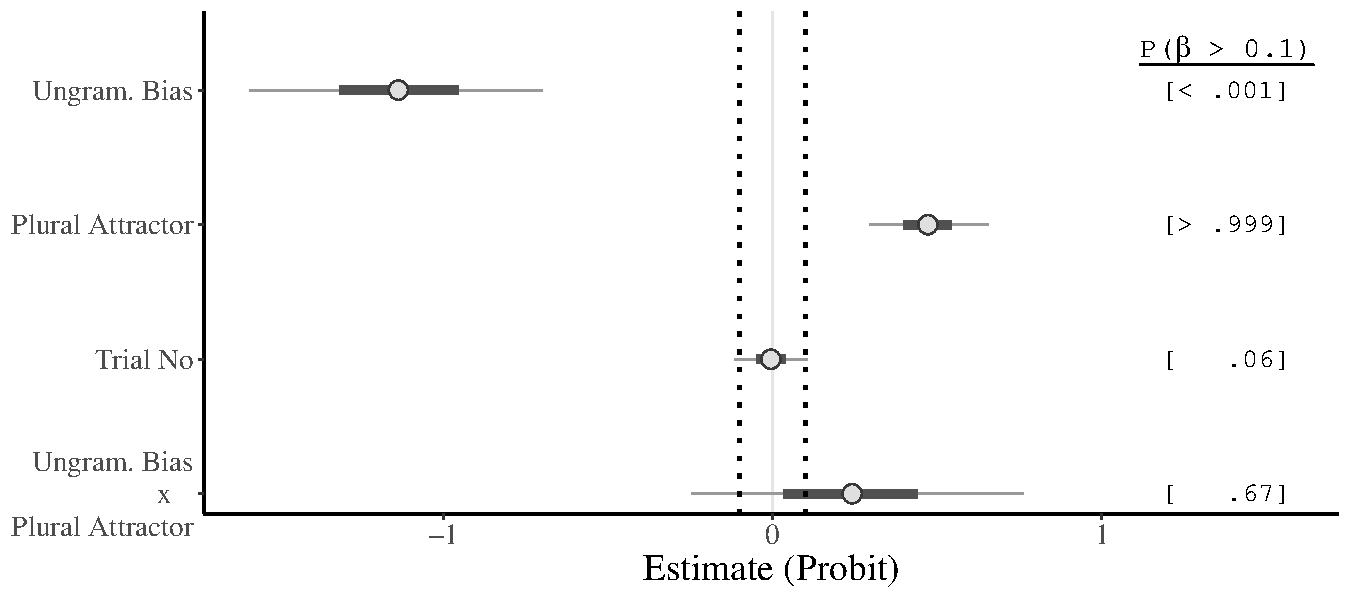
\includegraphics[width=\linewidth]{figure/UngramaticalBayesianGLM-1} 

}

\caption{Estimates and 95\% credible intervals for the probit regression coefficients for the model of responses to ungrammatical sentences in our Experiment 3}\label{fig:UngramaticalBayesianGLM}
\end{figure}

\end{knitrout}


Figure \ref{fig:GrammaticalBayesianGLM} shows the posterior distributions of a Bayesian GLM with grammatical sentences alone. The main effect of ungrammaticality bias ($\hat{\beta}=-0.24;$ $CI=[-0.79; 0.31];$ $P(\beta< -0.1)=    .69$) was relatively weak, meaning that we cannot definitively say participants found grammatical sentences more acceptable as their bias is shifted towards ungrammatical answers. This effect, again, verified that our bias calculation was on the right track. 

Meanwhile, the main effect of the plural attractor in grammatical sentences ($\hat{\beta}=-0.22;$ $CI=[-0.51; 0.04];$ $P(\beta< -0.1)=    .82$) tells us that with an average response bias, participants give less acceptable responses with a substantially higher probability when a plural attractor is present. Given that the average bias in our experiment is 0.06, which corresponds to a neutralized grammaticality bias, we can say that the apparent main effect of the plural attractor is an indicator of agreement attraction effects in grammatical sentences. Moreover, the negative interaction between the ungrammaticality bias and the presence of a plural attractor ($\hat{\beta}=-0.47;$ $CI=[-1.09; 0.17];$ $P(\beta< -0.1)=    .87$) tells us that participants with an ungrammaticality bias are even more affected by the presence of a plural attractor in grammatical sentences. 

\begin{knitrout}
\definecolor{shadecolor}{rgb}{0.969, 0.969, 0.969}\color{fgcolor}\begin{figure}[hbt!]

{\centering 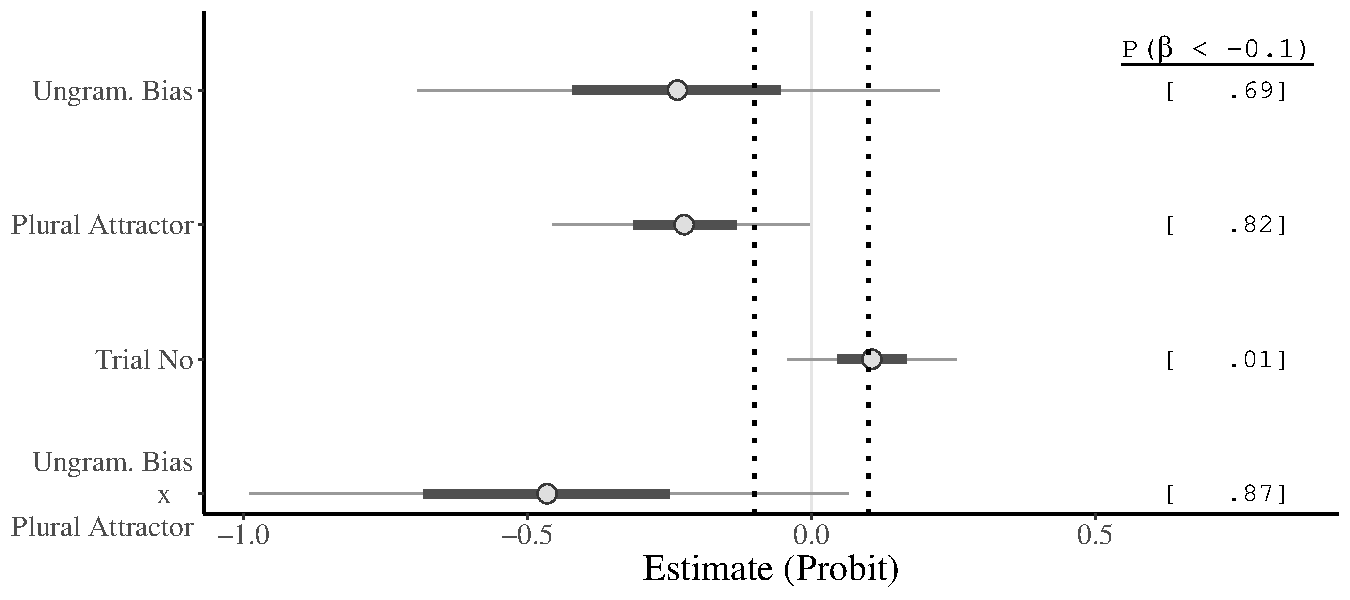
\includegraphics[width=\linewidth]{figure/GrammaticalBayesianGLM-1} 

}

\caption{Estimates and 95\% credible intervals for the probit regression coefficients for the model of responses to grammatical sentences in our Experiment 3}\label{fig:GrammaticalBayesianGLM}
\end{figure}

\end{knitrout}

Taken together, our results suggested that the bias shift towards ungrammatical responses, which we calculated using the filler items, reduced overall acceptable responses in ungrammatical experimental items as expected in the drift-diffusion model. In addition, we have moderate evidence that tells us that ungrammaticality bias affects acceptable responses in grammatical sentences. With an average bias, the probability of giving acceptable responses is reduced substantially with plural attractors in grammatical sentences compared to sentences with singular attractors in grammatical sentencens, creating an ungrammaticality illusion. However, we can say that the effect of the plural attractor is more pronounced in people with ungrammaticality bias in grammatical sentences than in ungrammatical sentences. This emphasizes that the ungrammaticality illusion that we observe in grammatical sentences with plural attractors is amplified in a continuous manner as bias shifts towards more and more ungrammatical responses as expected by the drift-diffusion model.

\section{Discussion}

This chapter re-examined \cites{HammerlyEtAl2019} findings. It also tested the predictions of the drift-diffusion model in agreement attraction: an amplified effect of plural attractor in grammatical sentences with a decreased bias towards grammatical responses. 
Suppose readers are biased to find sentences grammatical more often than ungrammatical, and lack of agreement attraction effects in grammatical sentences is due to this fact. 
In that case, they should be making more errors in grammatical sentences with plural attractors when their bias towards grammatical responses is neutralized or reversed. 

To this end, we conducted a speeded acceptability judgment experiment (N=114) with two within-subject factors (Attractor number x Verb number: 2x2) and a between-subject factor Bias. 
Following \citeand{HammerlyEtAl2019}, we manipulated the response bias utilizing instructions and the ratio of ungrammatical fillers. 
Our results can be summarized as follows. 
Our participants did not respond to the bias manipulation uniformly, and the effect of the instructions and the ratio of ungrammatical sentences was not significant. 
When we calculated the response bias following \citeand{MacmillanCreelman2005} and used it in our Bayesian GLM as a continuous predictor, 
we saw that the presence of a plural attractor substantially reduced the acceptable responses in grammatical responses as well.  
This effect of the plural attractor was even more amplified when the participants had a bias towards ungrammatical answers.

Based on the participants' response profile and our simulation results, we can say that our findings were parallel with those of previous studies that showed processing difficulty in grammatical sentences with plural attractors as differences in response times or acceptable responses.
Furthermore, our results show that attraction in grammatical sentences may emerge as a difference in acceptable responses, following from accounts of attraction that rely on feature percolation and faulty encoding of subjects \citep[][among others]{EberhardEtAl2005}.

These findings present a challenge for retrieval accounts \citep{LagoEtAl2015, LagoEtAl2019, WagersEtAl:2009}, which argue that for participants, the plurality of the attractor is only relevant in ungrammatical sentences, which is only when they may consider other DPs as a possible controller. 
Since attractor, be it single or plural, does not come into play unless the sentence is ungrammatical, these accounts predict that participants' bias should not affect the acceptability in grammatical sentences. 
Thus, the lack of a significant interaction between the grammaticality and the plural attractor in most studies suggested that retrieval accounts may capture agreement attraction effects better (Schlueter, Parker, \& Lagu, 2019; Hammerly et al., 2019; Lago et al., 2021). 

However, when bias is accounted for, it seems that grammaticality asymmetry is not due to the nature of how subject-verb dependency is processed as argued before by the retrieval accounts \citep[][among others]{WagersEtAl:2009}, but a direct residue of how participants make decisions in forced-choice experiments. 

What is still left as an intriguing issue is that neither \citeand{HammerlyEtAl2019} nor we could introduce a bias manipulation according to the response bias values calculated through filler items. Despite this fact, their results from Experiment 3 exhibit an apparent effect of plural attractor in grammatical and ungrammatical sentences. These results would be expected only if their bias manipulation were successful.

To sum up, we attempted to replicate \cites{HammerlyEtAl2019} study in Turkish with a different syntactic construction: a noun phrase with a genitive modifier. We argued that response bias shift might result in ungrammaticality illusion in another language with a structure that was found to be attraction-vulnerable \citep{LagoEtAl2015}. We presented our speeded acceptability judgment task results which showed comparable results with \citeand{HammerlyEtAl2019}. While we could not manipulate participants' response bias, we replicated the theoretical claims of \citeand{HammerlyEtAl2019}. We confirmed the predictions of the Marking \& Morphing account implemented with the drift-diffusion model. We argue that cue-based retrieval models cannot account for the role of the response bias in agreement attraction, which we demonstrated. 
